\documentclass[a4paper,11pt,oneside]{book}
\usepackage[T1]{fontenc}
\usepackage[utf8]{inputenc}
\usepackage[english]{babel}
\usepackage[a4paper,top=2cm,bottom=2cm,left=3cm,right=2cm]{geometry}
\usepackage{graphicx}
\usepackage{amsmath,amssymb}
\usepackage{booktabs}
\usepackage{array}
\usepackage{enumitem}
\usepackage{xcolor}
\usepackage{listings}
\usepackage{microtype}
\usepackage[numbers,sort&compress]{natbib}
\usepackage[hidelinks]{hyperref}

\linespread{1.25}
\emergencystretch=1em
\graphicspath{{img/}}
\setlist[itemize]{itemsep=0.35em}
\lstset{
  basicstyle=\ttfamily\small,
  breaklines=true,
  frame=single,
  columns=fullflexible,
  showstringspaces=false
}

\begin{document}
\begin{titlepage}
\centering
\vspace*{0.4cm}

\includegraphics[width=2.7cm]{unisalento-logo.png}\par
\vspace{0.5cm}
{\Large UNIVERSITY OF SALENTO\par}
\vspace{0.4cm}
{\Large FACULTY OF ENGINEERING\par}
\vspace{0.4cm}
{\large BACHELOR'S DEGREE IN COMPUTER ENGINEERING\par}
\vspace{0.8cm}
\rule{0.9\textwidth}{0.4pt}
\vspace{1.2cm}
{\Large THESIS IN ARTIFICIAL INTELLIGENCE\par}
\vspace{1cm}
{\LARGE\bfseries Probabilistic Three-Dimensional Forecasting of the Ocean State in the Mediterranean Sea Using 3D U-Net Neural Networks\par}
\vfill
\begin{minipage}{0.45\textwidth}
\raggedright
\textbf{Supervisor:}\\
Prof. Italo Epicoco
\end{minipage}
\hfill
\begin{minipage}{0.45\textwidth}
\raggedleft
\textbf{Candidate:}\\
Arturo Marino\\
Student ID: 20089080
\end{minipage}
\vfill
{\large ACADEMIC YEAR 2025/2026\par}
\end{titlepage}

\frontmatter
\tableofcontents
\listoffigures
\listoftables
\mainmatter
\chapter{Introduction}
\label{chap:introduction}

\section{Background and Problem Statement}

Ocean forecasting is a central problem in environmental modelling, with direct relevance to climate analysis, marine safety, ecosystem monitoring, and the management of coastal and offshore activities. The ocean state evolves through coupled physical processes that act across a wide range of spatial and temporal scales. Temperature, salinity, sea level, and horizontal currents are not independent quantities: their interactions determine density gradients, circulation, stratification, and the transport of heat and matter. A forecast must therefore represent both horizontal variability and changes along the water column.

Operational ocean forecasting systems are primarily based on numerical models that discretize and integrate the governing equations of ocean dynamics. These systems provide physically consistent predictions and remain essential in scientific and operational settings. Their use, however, requires substantial computational resources, carefully specified surface and lateral boundary conditions, and data-assimilation procedures that combine models with observations. These requirements motivate research into data-driven approaches that learn predictive relationships directly from historical ocean states and can produce forecasts at a lower inference cost.

Deep learning has recently achieved important results in geophysical forecasting \citep{bi2023pangu,lam2023graphcast}. Neural networks can learn complex spatio-temporal relationships from large reanalysis archives, while convolutional and encoder--decoder architectures are naturally suited to gridded fields. Applying these methods to the ocean remains difficult \citep{epicoco2026medformer}. Coastlines create irregular boundaries inside a rectangular grid, bathymetry changes the valid domain with depth, observations below the surface are comparatively sparse, and the short-term evolution can be much smaller than the absolute value of the state being predicted. At a one-day horizon, the simple persistence forecast---copying the last observed state---is consequently a demanding baseline.

This thesis investigates short-term, three-dimensional ocean-state forecasting over the Mediterranean region using a probabilistic neural network. The implemented model is a compact 3D U-Net trained on a Copernicus Marine GLORYS12-derived NetCDF subset \citep{copernicusglorys12,lellouche2021glorys12}. It receives three consecutive daily states and predicts the following daily state for potential temperature, salinity, and the two horizontal current components. In addition to a predictive mean, the network estimates a spatially varying Gaussian variance. The resulting system can therefore be evaluated both as a deterministic forecaster and as a model of conditional predictive uncertainty.

\section{Thesis Objectives}

The main objective is to design, implement, and evaluate a reproducible deep-learning pipeline for probabilistic ocean forecasting. The work covers the complete experimental path from large NetCDF files to quantitative validation. Its specific objectives are:

\begin{itemize}
  \item to load and preprocess Copernicus Marine data with Xarray and Dask while avoiding the materialization of the complete archive in memory;
  \item to represent temperature, salinity, eastward velocity, and northward velocity as multi-channel three-dimensional PyTorch tensors;
  \item to construct temporally ordered supervised samples without leakage between training, validation, and test years;
  \item to implement a 3D U-Net that predicts the mean and log-variance of the next ocean state;
  \item to train the network with a masked probabilistic objective that excludes land and missing values;
  \item to quantify deterministic accuracy, forecast skill relative to persistence, and the empirical coverage of the predicted uncertainty intervals;
  \item to identify the main limitations of the resulting model and define technically justified directions for future development.
\end{itemize}

The sea-surface-height field is retained by the preprocessing pipeline but is not used by the volumetric forecaster. It is two-dimensional, whereas the selected temperature, salinity, and velocity variables are defined over depth. Replicating the surface field along the vertical dimension would create artificial information; a multi-branch architecture would be required to integrate it consistently.

The intended contribution is an experimentally traceable research prototype rather than a complete operational forecasting service. Particular attention is given to the choices that affect the interpretation of the results: chronological splitting, depth-dependent normalization, masking, checkpoint selection, comparison with persistence, and separation between deterministic error and probabilistic coverage.

\section{Thesis Structure}

Chapter~\ref{chap:state-of-art} reviews artificial-intelligence methods for atmospheric and ocean forecasting, including deterministic, ensemble, and generative approaches. Chapter~\ref{chap:architecture} describes the dataset, preprocessing, network architecture, loss function, training loop, and computational configuration. Chapter~\ref{chap:evaluation} presents the inference protocol, metrics, quantitative results, maps, and uncertainty diagnostics. Chapter~\ref{chap:conclusions} relates the experimental evidence to the initial objectives and discusses limitations and future developments.

\chapter{State of the Art}
\label{chap:state-of-art}

\section{From Numerical Models to Data-Driven Forecasting}

Atmospheric and ocean forecasting have traditionally been formulated as initial-value problems governed by systems of partial differential equations. Numerical prediction systems discretize those equations over a grid, estimate an initial state through data assimilation, and integrate the state forward in time. Their principal strength is physical consistency: conservation laws and parameterized physical processes constrain the evolution. Their principal cost is computational. Operational forecasts require large computing systems, repeated assimilation cycles, and ensembles when uncertainty must be quantified.

Machine-learning forecasting follows a different route. A model is trained on archives of consecutive geophysical states and learns an approximation of the time-evolution operator. Once trained, inference consists mainly of tensor operations and can be much faster than a numerical integration. The learned mapping, however, is determined by the training distribution and objective. It may violate physical relationships, smooth small-scale structures, or accumulate errors when applied autoregressively. For this reason, comparisons with strong numerical or statistical baselines and temporally independent test periods are essential.

Reanalysis products have enabled much of the recent progress. A reanalysis combines a numerical model with historical observations to generate a spatially and temporally consistent record. It supplies the dense gridded targets required by supervised learning, but it is not identical to direct observation. A neural forecast trained and evaluated against reanalysis therefore learns to emulate the reanalysis state and inherits part of its uncertainty and bias. Independent observations remain valuable for operational validation, as illustrated by recent regional ocean systems.

\section{Artificial Intelligence for Atmospheric Forecasting}

The atmosphere has provided the most visible demonstrations of global data-driven forecasting. Large reanalysis archives, regular pressure-level representations, and established benchmarks make it possible to train and compare high-capacity models over many variables and lead times.

\subsection{FourCastNet}

FourCastNet introduced a global high-resolution weather model based on Adaptive Fourier Neural Operators. Rather than relying exclusively on local convolutional kernels, the architecture performs part of its computation in spectral space, allowing long-range spatial interactions to be represented efficiently. The model was trained on ERA5 fields at a horizontal resolution of $0.25^{\circ}$ and applied autoregressively to short- and medium-range forecasts \citep{pathak2022fourcastnet}. Its results showed that a neural model can produce global forecasts rapidly enough to support large ensembles.

FourCastNet is relevant to ocean forecasting for two reasons. First, it treats prediction as the learning of an evolution operator over gridded physical fields. Second, its autoregressive use highlights the difference between one-step accuracy and long-horizon stability. A small one-step bias can grow over repeated applications, so evaluation must consider the intended forecast horizon rather than assuming that a good single step guarantees a stable trajectory.

\subsection{Pangu-Weather}

Pangu-Weather introduced a three-dimensional Earth-specific transformer that represents pressure levels as an explicit spatial dimension. The model combines this representation with a hierarchical temporal aggregation strategy based on networks trained for different lead-time increments \citep{bi2023pangu}. The three-dimensional formulation is particularly relevant to this thesis because it preserves interactions between vertical levels instead of processing each level as an unrelated two-dimensional map.

The result also illustrates the importance of inductive bias. Atmospheric grids are structured but not equivalent to ordinary images: latitude, longitude, and vertical level have different physical meanings. Pangu-Weather incorporates these distinctions in its architecture. The present work uses a much smaller convolutional model, but it follows the same broad principle by processing depth jointly with the two horizontal dimensions.

\subsection{GraphCast}

GraphCast represents the atmosphere on a multi-scale graph and learns message-passing operations between grid points and graph nodes. It predicts global states autoregressively and was evaluated against the ECMWF deterministic high-resolution system over a large set of variables and lead times \citep{lam2023graphcast}. The graph representation permits information to travel efficiently over long distances while retaining a mapping to the regular latitude--longitude grid.

GraphCast demonstrates that model architecture, training data, and evaluation protocol must be considered together. Its scale and global context differ greatly from the regional experiment in this thesis, yet its validation principles remain applicable: the test period must be temporally separated, the baseline must be competitive, and performance must be reported across variables rather than through a single visually convincing case.

\subsection{Probabilistic Atmospheric Models}

Most early neural weather models produced a single deterministic trajectory. This is insufficient when multiple future states are plausible. GenCast addresses this limitation with a conditional diffusion model that generates an ensemble of global weather trajectories. It produces 15-day forecasts at $0.25^{\circ}$ resolution and evaluates the resulting joint distribution rather than only an ensemble mean \citep{price2024gencast}. This distinction is important: a distribution over coherent fields contains spatial and temporal dependencies that cannot be recovered from independent pointwise variances alone.

The probabilistic formulation used in this thesis is more limited. It predicts the parameters of a Gaussian distribution independently at every output location and variable. This provides a tractable uncertainty estimate and supports likelihood-based training, but it does not generate spatially coherent alternative ocean evolutions. GenCast therefore represents a possible long-term direction rather than a feature of the implemented system.

\section{Artificial Intelligence for Ocean Forecasting}

Transferring data-driven forecasting from the atmosphere to the ocean is not direct. The ocean evolves more slowly, has an irregular wet domain that changes with depth, and is strongly constrained by bathymetry, coastlines, narrow straits, surface fluxes, and lateral boundary conditions. Subsurface observations are sparse compared with atmospheric observations, and reanalysis fields may reflect changes in the observing network. At short lead times, gradual evolution also makes persistence difficult to outperform.

Ocean models can be grouped by domain and forecast scale. Global systems learn basin-to-basin interactions and require very large training sets. Regional systems can devote capacity to a specific circulation regime and use higher resolution, but they depend more strongly on the treatment of lateral boundaries. Surface-only systems reduce dimensionality, while three-dimensional systems attempt to represent stratification and the coupling between surface and subsurface dynamics.

\subsection{OceanNet and XiHe}

OceanNet is a regional neural-operator approach for ocean circulation. It combines a Fourier neural operator with a predictor--evaluate--corrector integration strategy and a spectral regularizer intended to reduce small-scale spectral bias. Its experiments focus on sea-surface-height evolution in energetic western-boundary-current regions \citep{chattopadhyay2023oceannet}. The work shows how neural operators can support long integrations, although a surface variable alone does not represent the complete three-dimensional ocean state.

XiHe extends data-driven forecasting to a global, eddy-resolving ocean configuration. It is trained on GLORYS12 reanalysis data and uses a hierarchical transformer architecture to forecast multiple ocean variables on a $1/12^{\circ}$ grid \citep{wang2024xihe}. Compared with a compact regional U-Net, XiHe benefits from a much larger archive, broader spatial context, and substantially greater model capacity. Its use of an explicit ocean mask and a three-dimensional dataset nevertheless addresses several of the same representation problems encountered in this thesis.

\subsection{Mediterranean Forecasting and MedFormer}

The Mediterranean Sea is a demanding regional domain. Its circulation is affected by complex coastlines, strong mesoscale activity, exchanges through narrow straits, and interactions between surface forcing and vertical stratification. A rectangular data array contains a large fraction of land cells and also includes boundary regions outside the basin, making masking and domain definition important.

MedFormer is a fully data-driven system developed specifically for medium-range forecasting in the Mediterranean Sea. Its architecture combines a U-Net with three-dimensional attention mechanisms. It operates at $1/24^{\circ}$ horizontal resolution, is pretrained on a long reanalysis archive, fine-tuned with operational analyses, and produces nine-day forecasts autoregressively. Historical ocean states are combined with atmospheric forcing, and evaluation includes comparison with the operational Mediterranean Forecasting System and independent observations \citep{epicoco2026medformer}.

MedFormer is the closest methodological reference for the present thesis, but the two systems have different aims. MedFormer targets operational medium-range performance at high resolution. The implemented 3D U-Net is a compact research prototype trained on a six-year subset, uses only four ocean variables, predicts one day ahead, and represents uncertainty with pointwise Gaussian parameters. This narrower design makes the complete pipeline manageable within the available computational resources and exposes the effects of masking, normalization, loss construction, and baseline choice.

\section{Architectural Families for Gridded Geophysical Data}

The models reviewed above use markedly different internal representations. This is more than an implementation detail: an architecture determines how information travels across space, how resolution affects cost, and which physical structures are easy or difficult to represent. Four broad families are relevant to the present work.

\subsection{Convolutional Encoder--Decoder Networks}

Convolutional networks apply shared local filters across a grid. Weight sharing makes them comparatively parameter-efficient, and a hierarchy of downsampling operations increases the receptive field without applying a large kernel at full resolution. Encoder--decoder networks then recover the original grid size, while skip connections transfer fine-scale information around the compressed representation. The U-Net design was introduced for image segmentation, where output localization is as important as global context \citep{ronneberger2015unet}. Its three-dimensional extension replaces planar operations with volumetric convolutions and was originally proposed for dense volumetric segmentation \citep{cicek20163dunet}.

Those properties transfer naturally to ocean forecasting. Temperature, salinity, and velocity are defined on a common grid, and a dense output is required for every wet cell. Three-dimensional kernels can combine neighbouring depths with horizontal information and therefore offer a direct way to represent stratification. Skip connections can preserve coastline and frontal detail that might otherwise be lost in the latent representation.

Convolutional U-Nets also have limits. Their translation-equivariant filters do not know that the same local pattern has a different meaning near Gibraltar, in the Adriatic Sea, or in the open eastern Mediterranean unless coordinates or static fields are supplied. Their receptive field grows only with depth, kernel size, and downsampling. Long-range teleconnections or basin-scale pressure gradients may therefore require a deeper network, attention, or operator-based components. Pooling can also smooth energetic small-scale structures, particularly when the target is a conditional mean.

\subsection{Neural Operators}

Neural operators aim to learn mappings between functions rather than mappings tied to one finite vector representation. Fourier neural operators transform fields into spectral space, modify a truncated set of modes, and return to physical space \citep{li2021fno}. A spectral layer can transmit information globally in a small number of operations, which motivated its use in FourCastNet and OceanNet.

For geophysical forecasting, global mixing is attractive because large-scale structures span many grid cells. At the same time, truncating high-frequency modes may reduce sharp fronts, coastally trapped signals, or energetic eddies. Irregular ocean masks also complicate the meaning of a global Fourier basis: discontinuities at land boundaries can create spectral artefacts. Hybrid designs can combine spectral processing for large scales with local convolutions or correction terms for smaller scales.

\subsection{Transformers and Attention}

Attention allows each representation element to combine information from other elements with data-dependent weights. A fully global attention matrix over a three-dimensional ocean grid is prohibitively large, so practical systems use windows, hierarchies, factorization, or sparse neighbourhoods. Pangu-Weather and XiHe use hierarchical designs, while MedFormer introduces 3D attention inside a regional encoder--decoder structure.

Compared with a fixed convolutional kernel, attention can adapt its spatial relationships to the current state. It may connect distant regions or depths when their features are relevant to the forecast. Its cost and data requirements are higher, however, and positional information must be encoded carefully. In a small six-year experiment, a compact convolutional baseline is useful before introducing a larger attention module because it separates limitations caused by data and objective from those caused by insufficient architectural capacity.

\subsection{Graph and Mesh Representations}

Graph networks replace rectangular neighbourhoods with an explicit connectivity structure. GraphCast maps regular atmospheric fields to a multi-resolution spherical mesh, performs message passing, and maps the result back to the grid. For the ocean, a graph can in principle exclude land connections, follow an unstructured coastal mesh, and represent narrow passages more faithfully than a rectangular convolution.

This flexibility introduces additional design decisions. Nodes, edges, distances, bathymetry, and the relation between depth levels must be specified, while efficient batching and interpolation become more complex. A graph is therefore attractive for a future physically informed model but is outside the scope of the implemented regular-grid pipeline.

\begin{table}[htbp]
\centering
\small
\caption{Representative data-driven geophysical forecasting systems. Resolutions and horizons refer to the configurations reported in the cited publications.}
\label{tab:state-of-art-models}
\begin{tabular}{p{2.2cm}p{2.2cm}p{3.1cm}p{2.1cm}p{2.2cm}}
\toprule
Model & Domain & Main architecture & Resolution & Output type \\
\midrule
FourCastNet & Global atmosphere & Adaptive Fourier neural operator & $0.25^{\circ}$ & Deterministic; ensembles through perturbed inputs \\
Pangu-Weather & Global atmosphere & 3D Earth-specific transformer & $0.25^{\circ}$ & Deterministic \\
GraphCast & Global atmosphere & Multi-scale graph neural network & $0.25^{\circ}$ & Deterministic \\
GenCast & Global atmosphere & Conditional diffusion model & $0.25^{\circ}$ & Probabilistic ensemble \\
OceanNet & Regional ocean & Fourier neural operator with correction step & Regional configuration & Deterministic autoregressive \\
XiHe & Global ocean & Hierarchical transformer & $1/12^{\circ}$ & Deterministic \\
MedFormer & Mediterranean Sea & U-Net with 3D attention & $1/24^{\circ}$ & Deterministic autoregressive \\
This thesis & Mediterranean subset & Compact probabilistic 3D U-Net & $0.25^{\circ}$ local grid & Pointwise Gaussian \\
\bottomrule
\end{tabular}
\end{table}

\section{Global and Regional Forecasting Strategies}

Global and regional models solve related but distinct problems. A global ocean model avoids artificial lateral boundaries and can learn connections between basins. It also requires a vast grid, substantial model capacity, and a long archive to represent the diversity of global regimes. XiHe follows this strategy at eddy-resolving resolution. Global atmospheric systems benefit similarly from complete spherical context, although they must handle the pole and periodic longitude explicitly.

A regional model restricts computation to a chosen area and can allocate more resolution or model capacity to that domain. It can learn recurring structures specific to the region, and its smaller tensor size makes experiments feasible on limited hardware. The disadvantage is incomplete physical context. Water, heat, and momentum cross the open boundary, and their future values are not determined solely by the internal regional state. The rectangular subset used in this thesis includes an Atlantic sector west of Gibraltar, which provides some context for the Mediterranean exchange, but it does not supply explicit time-dependent boundary forcing.

The distinction also affects evaluation. A global average can hide large regional errors, while a regional average can be dominated by one sub-basin or by the distribution of wet cells with depth. Results should therefore identify the domain, mask, and aggregation dimensions. Comparisons between models at different resolutions or domains cannot be reduced to one RMSE without accounting for their variables, targets, lead times, and reference datasets.

Another difference concerns operational inputs. A research experiment commonly starts from consecutive reanalysis states. An operational forecast starts from an analysis available in near real time and also receives future atmospheric forcing and boundary conditions. MedFormer includes atmospheric predictors and operational fine-tuning, whereas the present model uses ocean history only. This gap is central when interpreting performance: the compact model is evaluated as a controlled emulator of one-day reanalysis evolution, not as a replacement for a complete operational chain.

\section{Evaluation Practices in Geophysical Forecasting}

Forecast evaluation must match the intended use. One-step training loss alone is not an adequate performance report. Deterministic models are commonly assessed with RMSE, MAE, anomaly correlation, spectral diagnostics, and variable-specific physical errors. Probabilistic models require proper scores and calibration diagnostics \citep{gneiting2007scoring}. Autoregressive models also need error as a function of lead time because small one-step errors can compound into unstable trajectories.

Baselines are equally important. Climatology tests whether a model uses the current state, while persistence tests whether it predicts change beyond the latest observation. Numerical operational systems provide a much stronger reference but may not be available on exactly the same grid and dates. At one day, persistence is especially competitive in the ocean. At longer horizons it gradually loses skill, so the ranking of two methods can depend on forecast lead time.

Masks and weighting can change the meaning of an aggregate score. A simple mean over all depth cells gives greater influence to levels and regions with more valid points. Area weighting is required on a latitude--longitude grid when cells represent different surface areas, and volume weighting would additionally account for vertical layer thickness. The evaluator in this thesis masks invalid points but does not apply cell-area or layer-thickness weights. Its aggregate metric is therefore a pointwise grid average in standardized space. This is sufficient for internally consistent checkpoint comparison, but it is not a volume-integrated physical error.

Finally, reanalysis-based evaluation measures agreement with a model-assimilation product, not direct truth. Independent profiles, satellite products, drifters, floats, and tide gauges can expose biases shared by the training and target reanalysis. MedFormer demonstrates the value of including observation-based verification in a regional system. Such data are outside the current experiment, so the claims in this thesis are limited to forecasting the supplied Copernicus-derived fields.

\section{Probabilistic Forecasting and Predictive Uncertainty}

A deterministic model estimates one future field, commonly interpreted as a conditional mean. It cannot describe whether a forecast is associated with low or high uncertainty. Ensemble methods instead generate several plausible trajectories, while parametric methods predict the parameters of a chosen probability distribution. Generative models can represent more complex, multimodal distributions at a higher computational and methodological cost.

The implemented network follows the parametric approach. For each valid output element it predicts a mean $\mu_i$ and a log-variance $s_i=\log\sigma_i^2$. The variance is heteroscedastic because it changes with the input and with the output position. The training loss rewards accurate means while penalizing variance estimates that are inconsistent with the observed residuals. This uncertainty is conditional on the model and data representation and is best interpreted as an aleatoric or residual uncertainty estimate. It does not quantify epistemic uncertainty caused by limited training data, parameter uncertainty, or architectural misspecification \citep{kendall2017uncertainties}.

The predicted distribution is also factorized: conditional covariances between variables, depths, and neighbouring grid points are not represented explicitly. Empirical coverage can test whether marginal intervals contain the expected fraction of targets, but it cannot establish that sampled three-dimensional fields would be dynamically coherent. A complete probabilistic evaluation would additionally consider proper scoring rules, sharpness, reliability across subsets, and multivariate dependence.

\section{Positioning of This Thesis}

The reviewed literature shows a progression from deterministic one-step emulators to global autoregressive systems and probabilistic generative ensembles. It also shows that strong results depend on large training archives, domain-specific representations, exogenous forcing, and rigorous evaluation. The present work addresses a smaller but complete problem: constructing a reproducible end-to-end pipeline for next-day three-dimensional prediction and testing whether a compact probabilistic U-Net can improve over persistence.

Its methodological contribution is the integration of lazy NetCDF access, depth-dependent standardization, chronological splitting, masked volumetric learning, heteroscedastic Gaussian output, resumable checkpointing, and baseline-based evaluation in a single implementation. The experiments do not claim operational superiority. Their value lies in establishing a verified baseline, identifying where the current architecture succeeds or fails, and defining the changes required for a stronger future model.

\chapter{Implemented Architecture}
\label{chap:architecture}

\section{System Overview}

The implemented system transforms a multi-year archive of daily ocean analyses into one-day-ahead probabilistic forecasts. The pipeline is deliberately modular: data access, physical-domain masking, temporal splitting, standardization, sample construction, neural inference, optimization, and evaluation are implemented as separate stages. This separation reduces the risk of data leakage and makes it possible to reproduce an inference run from a saved checkpoint without retraining the model.

Figure~\ref{fig:implemented-pipeline} reports only the operations that are present in the source code. In particular, the preprocessing stage selects variables and applies the land--sea mask. It does not resample the grid, smooth the fields, or construct derived physical features. The probabilistic objective is a Gaussian negative log-likelihood combined with a weighted mean-squared-error term; the Continuous Ranked Probability Score is not used.

\begin{figure}[htbp]
\centering
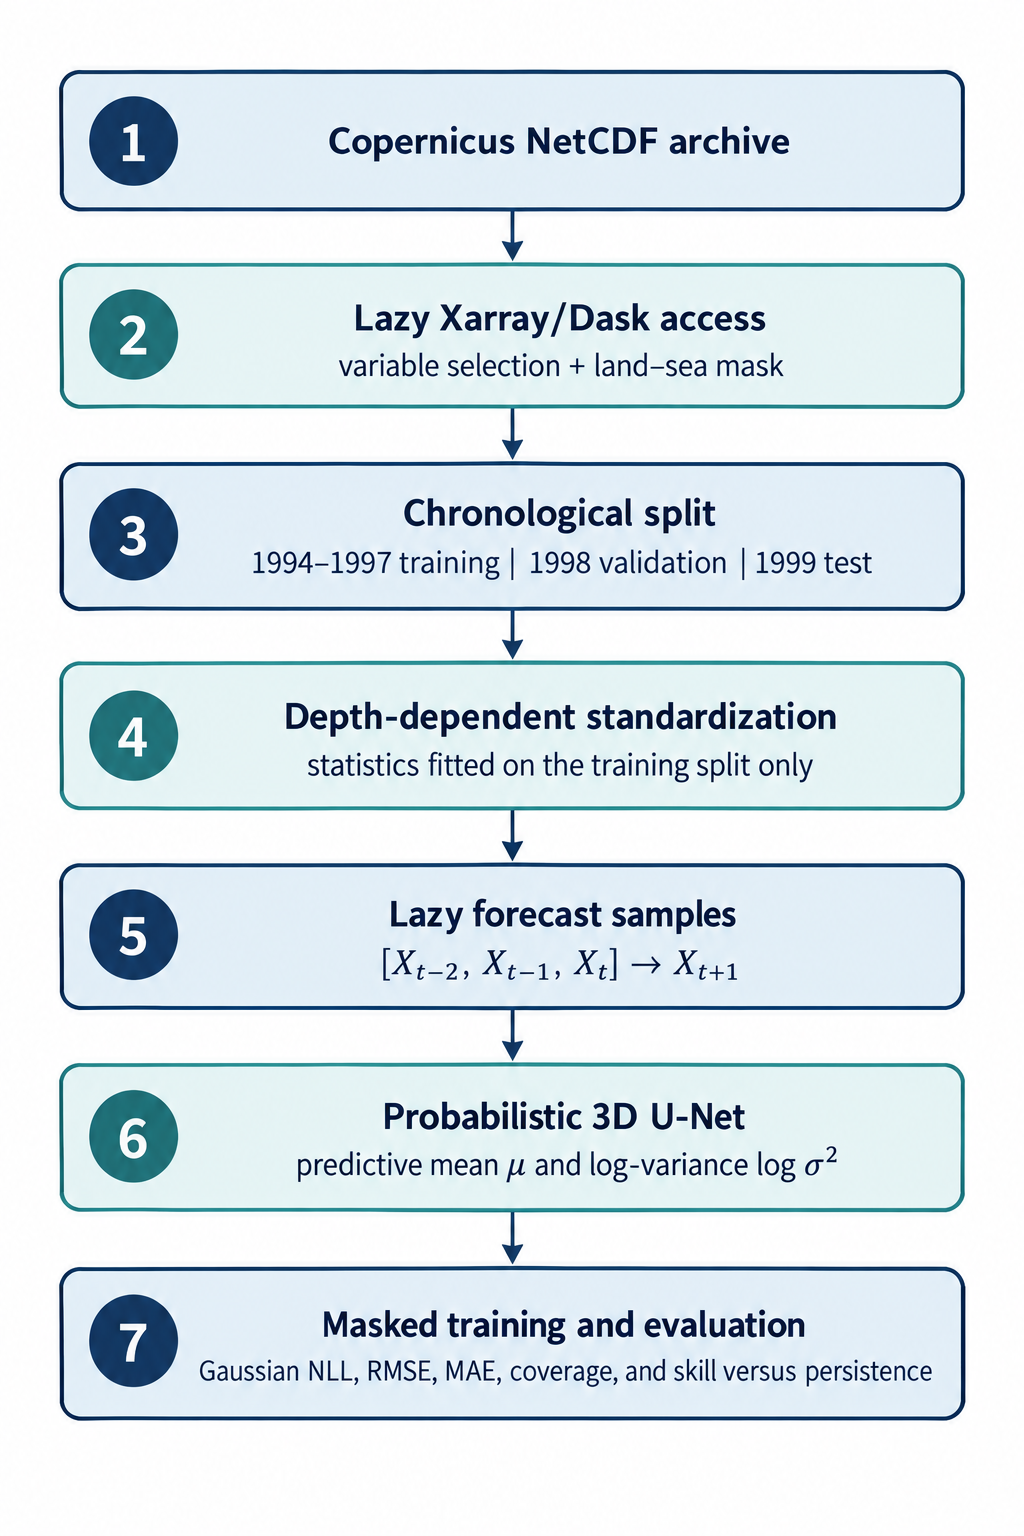
\includegraphics[width=0.82\textwidth]{implemented-pipeline.png}
\caption{Implemented data and modelling pipeline. The diagram excludes operations that are not present in the implementation.}
\label{fig:implemented-pipeline}
\end{figure}

The volumetric forecaster uses four variables: potential temperature, salinity, eastward velocity, and northward velocity. A fifth selected field, sea-surface height, is processed and standardized but remains outside the 3D network because it has no depth dimension. The implementation keeps this distinction explicit instead of repeating the same two-dimensional surface value at every depth level.

\section{Dataset and Preprocessing}

\subsection{Source Product and Extracted Domain}

The experiments use daily mean fields derived from the Copernicus Marine GLORYS12 global ocean reanalysis, distributed as product \texttt{GLOBAL\_MULTIYEAR\_PHY\_001\_030} \citep{copernicusglorys12,lellouche2021glorys12}. GLORYS12 is an eddy-resolving global reanalysis with a native horizontal resolution of $1/12^{\circ}$ and 50 vertical levels. The NetCDF file used in this thesis is a coarser regional extraction. Consequently, the $0.25^{\circ}$ spacing reported below describes the local file supplied to the experiment and must not be confused with the native product resolution.

The extracted array contains 2,191 daily time steps from 1 January 1994 through 31 December 1999. Its dimensions are

\[
(T,D,H,W)=(2191,46,65,171),
\]

where $T$ denotes time, $D$ depth, and $H$ and $W$ the latitude and longitude axes. Latitudes extend from $30.0^{\circ}$N to $46.0^{\circ}$N and longitudes from $6.0^{\circ}$W to $36.5^{\circ}$E, both with a $0.25^{\circ}$ step. The 46 retained depth levels are non-uniformly spaced, from approximately $0.506$~m to $947.448$~m. The rectangular bounds include the Mediterranean Sea together with adjacent ocean cells and land points; therefore, geographic bounds alone do not define the valid forecasting domain.

Table~\ref{tab:dataset-variables} lists the fields selected by the preprocessing module. The first four have dimensions \texttt{(time, depth, latitude, longitude)} and form the input and target volumes. Sea-surface height has dimensions \texttt{(time, latitude, longitude)}. Other fields present in the original file, including mixed-layer depth and sea-ice variables, are not selected by the implemented preprocessing stage.

\begin{table}[htbp]
\centering
\small
\caption{Variables selected from the Copernicus-derived NetCDF file. Units follow the product metadata.}
\label{tab:dataset-variables}
\begin{tabular}{llll}
\toprule
NetCDF name & Physical quantity & Unit & Use in 3D model \\
\midrule
\texttt{thetao\_cglo} & Potential temperature & $^{\circ}$C & Input and target \\
\texttt{so\_cglo} & Sea-water salinity & $10^{-3}$ & Input and target \\
\texttt{uo\_cglo} & Eastward velocity & m\,s$^{-1}$ & Input and target \\
\texttt{vo\_cglo} & Northward velocity & m\,s$^{-1}$ & Input and target \\
\texttt{zos\_cglo} & Sea-surface height & m & Processed, then excluded \\
\bottomrule
\end{tabular}
\end{table}

The input archive is opened with Xarray and Dask using chunks along the time dimension. This avoids loading approximately 2,191 full three-dimensional states into memory at once. Lazy access is especially important because each volumetric variable contains more than 1.2 billion grid values before masking. A sample is materialized only when requested by the PyTorch dataset. At that boundary, the selected Xarray slice is converted to a contiguous \texttt{float32} NumPy array and then to a PyTorch tensor.

\subsection{Land--Sea Mask and Missing Values}

The Mediterranean coastline, islands, and bathymetry create an irregular valid domain. The preprocessing module opens a stored land--sea mask and applies it to each selected field with Xarray's \texttt{where} operation. Invalid cells become \texttt{NaN} in the lazy dataset. When a sample is materialized, finite values generate a Boolean validity mask; the corresponding \texttt{NaN} values in the numerical tensor are replaced by zero. The loss and evaluation routines subsequently use the Boolean mask, so the inserted zeros do not contribute as artificial ocean observations.

The target mask is applied independently at every output channel and depth. This is necessary because a geographic location can be valid near the surface and invalid below the local seabed. It also protects the objective from non-finite values. The loss implementation replaces invalid values before the exponential in the Gaussian likelihood, preventing masked extreme values from producing \texttt{NaN} gradients.

\subsection{Depth-Dependent Standardization}

The four target variables have different units and numerical ranges. Training directly on physical values would cause large-scale variables to dominate the gradient. The implementation therefore applies a $z$-score transformation. For a volumetric variable $c$ and depth level $d$, the statistics are

\begin{align}
\mu_{c,d} &= \operatorname{mean}_{t,\phi,\lambda} X_{c,t,d,\phi,\lambda},\\
\sigma_{c,d} &= \operatorname{std}_{t,\phi,\lambda} X_{c,t,d,\phi,\lambda},
\end{align}

where the reductions cover time, latitude, and longitude while ignoring missing values. Depth is deliberately preserved. The normalized field is

\[
\widetilde{X}_{c,t,d,\phi,\lambda}
=
\frac{X_{c,t,d,\phi,\lambda}-\mu_{c,d}}
{\sigma_{c,d}}.
\]

Thus, the implementation uses statistics specific to each depth level rather than one scalar mean and standard deviation per variable. This choice prevents the strong vertical gradient of temperature and other fields from being treated as random variation around a single global mean. For the two-dimensional sea-surface-height field, the reduction produces scalar statistics because no depth coordinate exists.

All statistics are fitted exclusively on the 1994--1997 training split. The same stored values are then applied to validation and test data. The standard deviation is replaced by one only when it falls below a numerical threshold of $10^{-8}$. Saving the statistics in a separate NetCDF file ensures that inference performs exactly the same transformation and does not accidentally use information from later years.

\subsection{Chronological Split}

The dataset is divided chronologically:

\begin{itemize}
  \item training: 1 January 1994--31 December 1997, 1,461 daily states;
  \item validation: 1 January--31 December 1998, 365 daily states;
  \item test: 1 January--31 December 1999, 365 daily states.
\end{itemize}

A random split would allow very similar consecutive states to appear in different subsets and would yield an unrealistically favourable estimate of generalization. The chronological organization instead emulates the intended use: prediction of future states from an archive that contains only earlier years. The DataLoader construction also checks that timestamps do not overlap between splits.

\subsection{Forecast Sample Construction}

Each supervised sample uses three consecutive daily states as context and the following state as target:

\[
[X_{t-2},X_{t-1},X_t] \longmapsto X_{t+1}.
\]

Each state contains the four volumetric variables. Concatenating three states along the channel axis produces 12 input channels, while the target contains four channels. After batching, the tensor layout is

\[
[B,C,D,H,W],
\]

with input shape $[B,12,46,65,171]$ and target shape $[B,4,46,65,171]$. This notation describes the role of each axis once; the actual dimensions are used again in Table~\ref{tab:architecture-layers} only to document how the network transforms them.

Because each sample needs three context days and one target day, the splits contain 1,458 training pairs, 362 validation pairs, and 362 test pairs. The first validation and test targets are constructed entirely inside their respective yearly split. This discards the final context days of the preceding year but makes the separation rule unambiguous.

\section{Probabilistic 3D U-Net}

\subsection{Encoder--Decoder Structure}

The forecaster is a compact three-dimensional U-Net. Every convolutional block contains two $3\times3\times3$ convolutions with unit padding and a GELU activation after each convolution. Unit padding preserves depth, latitude, and longitude inside a block. The encoder progressively enlarges the receptive field through two \texttt{MaxPool3D} operations with kernel and stride equal to two. Channel capacity increases from 8 to 16 and then to 32 latent channels.

The decoder restores the exact resolution of the corresponding encoder feature map through trilinear interpolation. Interpolation targets the stored skip-connection shape rather than assuming that every axis is divisible by two. This detail is required for the $46\times65\times171$ grid, whose latitude and longitude sizes are odd. The upsampled features are concatenated with the encoder features, and a two-convolution block fuses the result.

Two independent $1\times1\times1$ projections transform the final eight features into four output channels. The first predicts the normalized conditional mean $\mu$; the second predicts the log-variance $s=\log\sigma^2$. The log-variance projection is initialized with zero weights and biases, corresponding to an initial normalized variance of one. Predicting the logarithm avoids a direct positivity constraint on the raw network output, while the standard deviation used during evaluation is recovered as $\sigma=\exp(s/2)$.

\begin{table}[htbp]
\centering
\small
\caption{Layer sequence and tensor shapes for the final network. Batch size is omitted from the shapes.}
\label{tab:architecture-layers}
\begin{tabular}{p{2.5cm}p{4.2cm}p{3.2cm}r}
\toprule
Stage & Operation & Output shape & Parameters \\
\midrule
Input & Three days, four variables & $12\times46\times65\times171$ & 0 \\
Encoder 1 & Two $3^3$ convolutions, GELU & $8\times46\times65\times171$ & 4,336 \\
Encoder 2 & MaxPool3D, two convolutions & $16\times23\times32\times85$ & 10,400 \\
Latent block & MaxPool3D, two convolutions & $32\times11\times16\times42$ & 41,536 \\
Decoder 2 & Trilinear upsample, skip, convolutions & $16\times23\times32\times85$ & 27,680 \\
Decoder 1 & Trilinear upsample, skip, convolutions & $8\times46\times65\times171$ & 6,928 \\
Mean head & $1\times1\times1$ convolution & $4\times46\times65\times171$ & 36 \\
Log-variance head & $1\times1\times1$ convolution & $4\times46\times65\times171$ & 36 \\
\midrule
Total & & & \textbf{90,952} \\
\bottomrule
\end{tabular}
\end{table}

The final configuration does not include instance normalization inside the convolutional blocks. The inputs are already standardized with training statistics specific to each variable and depth. Additional instance normalization would recompute statistics for every sample and channel and could suppress changes in absolute field level that are physically meaningful for forecasting. Its absence is therefore a documented model choice rather than an omitted preprocessing step.

\subsection{Design Rationale and Computational Cost}

The use of 3D rather than 2D convolutions is motivated by the vertical structure of the target. A two-dimensional network could treat depth levels as channels, but then each kernel would mix all levels through channel weights while translating only in latitude and longitude. The meaning of depth adjacency would be implicit and fixed at the first layer. In the adopted formulation, a $3\times3\times3$ kernel moves explicitly through depth and can build progressively larger vertical features. The same operation is shared across the water column, which provides a stronger inductive bias for local vertical continuity.

The four physical variables are concatenated as channels because they are defined on the same depth and horizontal coordinates. A convolution can therefore learn joint features such as a temperature--salinity structure accompanied by a velocity pattern. Standardizing each variable and depth before concatenation is critical: without it, salinity and temperature magnitudes would differ markedly from current velocities and would determine the scale of early-layer activations.

The model contains only two downsampling stages. Deeper compression would enlarge the receptive field but would reduce the already modest vertical dimension from 46 levels and make reconstruction of shallow coastal structure more difficult. Two stages yield a latent grid of $11\times16\times42$, preserving an explicit three-dimensional representation. The 32 latent feature channels provide capacity for joint ocean patterns while keeping the parameter count and activations manageable in a Colab session.

One unbatched input tensor contains

\[
12\times46\times65\times171=6{,}134{,}760
\]

single-precision values, or approximately 23.4~MiB before masks and intermediate activations. The four-channel target requires approximately 7.8~MiB, and the mean and log-variance outputs together require about 15.6~MiB. Training memory is substantially higher because encoder features, decoder features, gradients, and AdamW moment estimates must also be retained. These values explain the conservative batch size of one even though the network has fewer than one hundred thousand parameters: activation memory, not parameter memory, dominates this dense volumetric task.

The two output heads share the complete encoder and decoder. This reduces cost and lets the variance estimate depend on the same features used for the mean. It can also couple their errors: if the shared representation omits a relevant process, both heads must compensate from the same limited information. A larger future system could use a wider variance head, but such complexity should be introduced only after the deterministic mean surpasses the reference baseline.

\subsection{What the Output Distribution Represents}

Conditioned on the three input states, the model assumes a factorized Gaussian distribution over all valid target elements:

\[
p(Y\mid X)=\prod_{i\in\Omega}
\mathcal{N}(y_i;\mu_i,\sigma_i^2),
\]

where $\Omega$ is the set of ocean cells selected by the target mask. Both $\mu_i$ and $\sigma_i$ vary with variable, depth, and horizontal position, so the distribution is heteroscedastic. The factorization means that the likelihood does not contain an explicit covariance between adjacent locations, depths, or variables. Convolutions allow the predicted parameters to depend on a local three-dimensional context, but the probability model itself still treats output residuals as conditionally independent.

This distinction limits the interpretation of uncertainty. The predicted standard deviation expresses residual uncertainty learned from the training data under a fixed architecture and fixed parameters. It does not by itself measure epistemic uncertainty about the weights, nor does it define spatially coherent alternative ocean states. Ensembles, Bayesian approximations, or generative models would be required to address those aspects.

\section{Training Objective}

\subsection{Masked Gaussian Negative Log-Likelihood}

The objective uses the Gaussian logarithmic score, a proper scoring rule \citep{gneiting2007scoring}. For each valid normalized target $y_i$, mean prediction $\mu_i$, and predicted log-variance $s_i$, the implemented negative log-likelihood is

\[
\mathcal{L}_{\mathrm{NLL}}
=\frac{1}{|\Omega|}\sum_{i\in\Omega}
\frac{1}{2}\left[(y_i-\mu_i)^2\exp(-s_i)+s_i\right].
\]

The constant $\tfrac{1}{2}\log(2\pi)$ is omitted because it does not alter the optimizer. The first term penalizes the squared residual relative to the predicted variance. A model cannot reduce this term simply by predicting a very large variance because the second term grows with $s_i$. Conversely, predicting a variance that is too small makes errors expensive through $\exp(-s_i)$. The objective therefore trains the two output heads jointly.

Masking is part of the definition of the loss. Only elements in $\Omega$ enter the sum and its denominator. This is different from averaging over a rectangular tensor after setting land values to zero, which would reward the model for predicting artificial zeros over a large portion of the domain.

\subsection{Weighted Mean Error Term}

Preliminary configurations optimized the likelihood but did not always reduce the mean forecast error sufficiently. The final objective therefore adds a masked channel-weighted mean-squared error:

\[
\mathcal{L}_{\mathrm{MSE}}
=
\frac{
\sum_{i\in\Omega} w_{c(i)}(y_i-\mu_i)^2
}{
\sum_{i\in\Omega} w_{c(i)}
},
\qquad
w_c=
\begin{cases}
2,& c=\text{temperature},\\
1,& \text{otherwise}.
\end{cases}
\]

The complete optimization objective is

\[
\mathcal{L}=\mathcal{L}_{\mathrm{NLL}}+2\,\mathcal{L}_{\mathrm{MSE}}.
\]

The coefficient of the auxiliary MSE and the internal temperature weight are both 2.0 in the final run. They play different roles: the first controls the balance between distribution fitting and mean accuracy, whereas the second gives temperature twice the relative contribution of each other channel inside the MSE term. Metrics reported after an epoch remain unweighted aggregate errors unless explicitly identified as temperature-only physical metrics.

\section{Training Procedure}

\subsection{Data Loading and Device Transfer}

Training uses a batch size of one and zero worker processes. These conservative settings avoid several NetCDF files being read concurrently and bound the memory needed for a $12\times46\times65\times171$ input. The training DataLoader shuffles sample order at the start of each epoch, whereas validation and test loaders retain chronological order. CUDA pinned memory is enabled when a CUDA device is selected. Each input volume, target volume, and target mask is transferred to the device immediately before the forward pass.

One optimization epoch follows this sequence for every batch:

\begin{enumerate}
  \item clear the AdamW gradients with \texttt{set\_to\_none=True};
  \item compute the mean and log-variance through the 3D U-Net;
  \item compute the masked Gaussian NLL and weighted MSE;
  \item backpropagate their combined objective;
  \item clip the global gradient norm to 1.0;
  \item update the parameters with AdamW.
\end{enumerate}

After the optimization pass, the code evaluates the complete training split again with fixed end-of-epoch weights. This second pass is intentional: metrics accumulated while weights are changing cannot be compared directly with validation metrics computed from one fixed model. A no-gradient pass is then performed over validation. RMSE, MAE, NLL, predicted standard deviation, interval coverage, and skill relative to persistence are accumulated from valid points only.

\subsection{Optimizer, Checkpoints, and Reproducibility}

The final checkpoint records an AdamW learning rate of $10^{-4}$ and weight decay of $10^{-4}$ \citep{loshchilov2019adamw}, with $\beta_1=0.9$, $\beta_2=0.999$, and $\epsilon=10^{-8}$. No learning-rate scheduler is used. The random seed exposed by the training command defaults to 42. The maximum epoch and early-stopping patience actually passed to the historical command were not stored in the checkpoint; reporting the current command-line defaults as historical values would therefore be unjustified.

Two checkpoint files serve different purposes. The \emph{best} file is overwritten whenever validation RMSE improves. The \emph{last} file is written after every epoch and stores model weights, optimizer state, metric history, best epoch, and the number of consecutive epochs without improvement. A resumed training command loads the last file and checks that model dimensions, context length, and loss weights agree with the saved configuration before continuing.

The final run completed 96 epochs. Its best validation RMSE occurred at epoch 94, and the last checkpoint records two subsequent epochs without improvement. This does not reveal the configured patience, but it proves that model selection and the final experimental evaluation use epoch 94 rather than epoch 96.

\subsection{Hyperparameter Refinement}

Three preserved checkpoint families document the progressive enlargement of temporal context and network capacity. Table~\ref{tab:checkpoint-comparison} reports only fields recovered from the checkpoint files. The v1 checkpoint does not contain a validation-RMSE field, so its selection statistic is not directly comparable with the later runs. The value labelled ``minimum NLL in history'' is also not necessarily the NLL at the RMSE-selected epoch: the code tracks the lowest NLL over all completed epochs while choosing the best checkpoint by RMSE.

\begin{table}[htbp]
\centering
\small
\caption{Verified checkpoint configurations used during model refinement.}
\label{tab:checkpoint-comparison}
\begin{tabular}{lrrrrrr}
\toprule
Run & Context & Input ch. & Base ch. & Latent ch. & Best epoch & Val. RMSE \\
\midrule
v1 & 1 & 4 & 4 & 8 & 66 & unavailable \\
v2 fast & 2 & 8 & 8 & 32 & 28 & 0.208207 \\
v3 final & 3 & 12 & 8 & 32 & 94 & 0.178346 \\
\bottomrule
\end{tabular}
\end{table}

The sequence shows that the final configuration combines three days of context with the larger 8--16--32 feature hierarchy. The observed validation RMSE decreases from v2 to v3. This comparison does not isolate a single causal hyperparameter because context length and earlier configuration choices changed between runs; it documents empirical refinement rather than a controlled ablation study.

\section{Learning Curves}

Figure~\ref{fig:learning-curves} contains the complete history of the final run. Only one copy is retained in the thesis. Both training and validation NLL decrease rapidly during the first epochs and then continue with marked short-term fluctuations. The validation RMSE falls from approximately 0.358 at epoch 1 to 0.178 at epoch 94. Training and validation curves remain close, providing no evidence of a large classical generalization gap between the first four years and 1998.

The more consequential observation is the comparison with persistence. Although neural RMSE improves throughout training, the horizontal validation-persistence level remains lower. The checkpoint at epoch 94 is therefore the best neural configuration according to the chosen selection rule, yet it does not outperform the one-day persistence forecast. Chapter~\ref{chap:evaluation} quantifies this result on both validation and test data.

\begin{figure}[htbp]
\centering
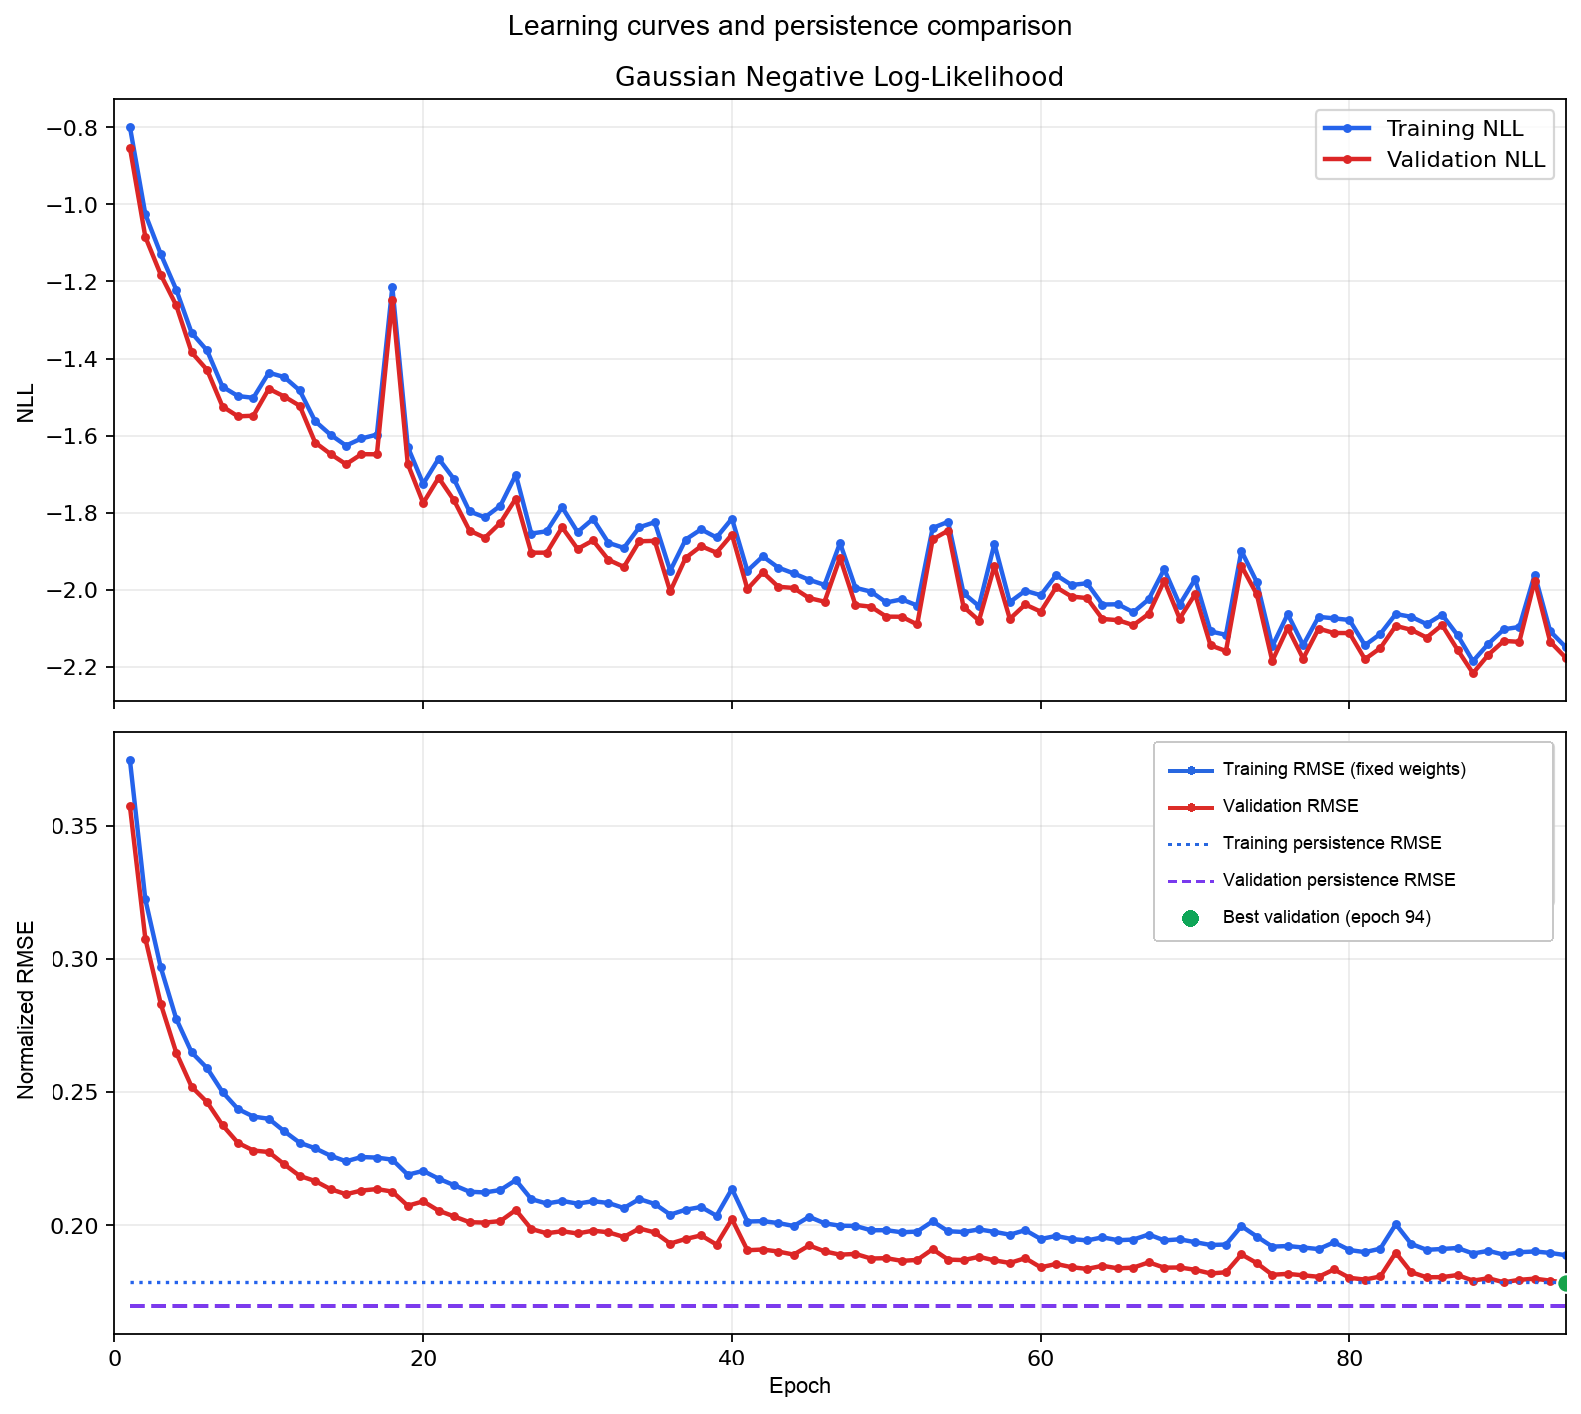
\includegraphics[width=0.96\textwidth]{learning-curve-english.png}
\caption{Gaussian NLL and normalized RMSE over the 96 completed epochs. Training metrics are recomputed with fixed end-of-epoch weights. Dotted lines show the persistence RMSE, and the marker identifies the RMSE-selected checkpoint at epoch 94.}
\label{fig:learning-curves}
\end{figure}

\section{Hardware, Software, and Runtime}

Training and inference were executed in Google Colab with CUDA acceleration. The checkpoint proves that 96 epochs were completed, including resumed sessions, but it does not store a GPU identifier, memory size, per-epoch timing, or accumulated wall-clock duration. The image files produced during development span multiple Colab sessions; their filesystem dates cannot be interpreted as continuous compute time. Consequently, the exact historical training GPU and total training time are unavailable and are not reconstructed from the currently assigned Colab hardware.

For reproducibility, a later audit of the notebook environment recorded Python 3.13.15, PyTorch 2.11.0 compiled for CUDA 12.8, Xarray 2025.12.0, and Dask 2026.1.1. That audit session was assigned an NVIDIA A100-SXM4-40GB with approximately 39.5~GiB of memory. These values describe the environment used to re-run inference and inspect checkpoints; they are not evidence that the same GPU or package versions were used for every historical training epoch. Future runs should write this metadata and elapsed time into the last checkpoint at every session boundary.

\chapter{Experimental Evaluation}
\label{chap:evaluation}

\section{Evaluation Protocol}

The experimental evaluation tests the ability of the selected model to forecast the next daily three-dimensional ocean state. Each inference sample contains three consecutive context days and one target one day after the final context state. All parameters are frozen during evaluation. The same preprocessing code, training-derived standardization statistics, variable order, and target masks used during training are restored before the network is called.

The best v3 checkpoint, selected at epoch 94 through validation RMSE, is evaluated on the complete 1998 validation year and the previously unseen 1999 test year. Because the model consumes three context days, the last two days of the preceding year are prepended to each evaluation period as inputs only. The first forecast uses 30--31 December and 1 January to predict 2 January; the last uses 28--30 December to predict 31 December. Thus each non-leap evaluation year contains 364 targets, all belonging to the year being evaluated. The chronological split itself was defined in Chapter~\ref{chap:architecture}; no target crosses a split boundary.

The aggregate evaluation can be reproduced with relative project paths using:

\begin{lstlisting}[caption={Inference commands for the selected checkpoint.}]
python src/train.py --data-path data/copernicus.nc \
  --mask-path data/masks/land_sea_mask.nc \
  --stats-path data/processed/normalization_stats.nc \
  --reuse-stats \
  --checkpoint-path checkpoints/best_forecaster_v3.pt \
  --evaluate-validation

python src/train.py --data-path data/copernicus.nc \
  --mask-path data/masks/land_sea_mask.nc \
  --stats-path data/processed/normalization_stats.nc \
  --reuse-stats \
  --checkpoint-path checkpoints/best_forecaster_v3.pt \
  --evaluate-test
\end{lstlisting}

The commands execute forward passes over an entire split; the appearance of a validation progress bar does not indicate that training has restarted. No optimizer is created for these evaluation branches and no gradient or parameter update is performed.

Physical-unit evaluation uses the same checkpoint for temperature, salinity, zonal velocity, and meridional velocity. The routine automatically chooses the closest level to the requested depth and reports both that slice and an aggregate over all depths. The same run also writes machine-readable JSON and CSV results and the annual error maps:

\begin{lstlisting}[caption={Annual physical-unit multivariable evaluation.}]
python src/train.py --data-path data/copernicus.nc \
  --mask-path data/masks/land_sea_mask.nc \
  --stats-path data/processed/normalization_stats.nc \
  --reuse-stats \
  --checkpoint-path checkpoints/best_forecaster_v3.pt \
  --evaluation-depth 0.5 \
  --evaluate-physical-validation \
  --evaluate-physical-test \
  --plot-annual-errors-test
\end{lstlisting}

The checkpoint is first loaded on the CPU so its configuration can define context length, channel dimensions, and internal normalization. The model is then constructed, weights are restored, and the complete object is moved to the selected evaluation device. This order prevents an inference command from silently evaluating a checkpoint with a model configuration taken from unrelated command-line defaults.

\section{Persistence Reference}

The neural forecast is compared with persistence. Given the latest input state $X_t$, persistence predicts

\[
\widehat{X}^{\mathrm{pers}}_{t+1}=X_t.
\]

This baseline has no trainable parameters and is evaluated over exactly the same targets, variables, depths, and masks as the neural model. It is particularly demanding at a 24-hour horizon because much of the ocean changes gradually. A neural model predicting the full state can achieve a low absolute error while still losing to persistence if it slightly smooths the input or introduces a small bias in regions that change little.

Persistence is more informative here than a constant climatology because it uses the most recent state available to the network. It also provides a direct test of whether the neural mapping has learned the daily increment rather than only the typical absolute state.

\section{Metrics and Aggregation}

Deterministic accuracy is measured from the predicted mean. For $N$ valid elements,

\begin{align}
\mathrm{RMSE} &= \sqrt{\frac{1}{N}\sum_{i=1}^{N}(y_i-\mu_i)^2},\\
\mathrm{MAE} &= \frac{1}{N}\sum_{i=1}^{N}|y_i-\mu_i|,\\
\mathrm{Bias} &= \frac{1}{N}\sum_{i=1}^{N}(\mu_i-y_i).
\end{align}

The normalized aggregate RMSE and MAE pool all four variables, all depths, all horizontal ocean points, and all dates of a split. They are dimensionless because every channel and depth has been standardized. Since such pooling can hide large differences among variables, residuals and predicted standard deviations are also converted back to the physical unit of each channel using the training standard deviation at the corresponding depth.

Skill relative to persistence is

\[
S_{\mathrm{RMSE}}=1-
\frac{\mathrm{RMSE}_{\mathrm{model}}^2}
{\mathrm{RMSE}_{\mathrm{pers}}^2}.
\]

A value above zero means that the neural mean has lower MSE than persistence; a value below zero means that persistence is more accurate. Because the score uses squared RMSE, even a modest difference between the two errors can produce a visibly negative value.

The probabilistic score is the masked Gaussian NLL defined in Chapter~\ref{chap:architecture}. It is not repeated algebraically here. Two marginal interval coverages complement it:

\begin{align}
C_{68} &= \frac{1}{N}\sum_i
\mathbf{1}(|y_i-\mu_i|\leq\sigma_i),\\
C_{95} &= \frac{1}{N}\sum_i
\mathbf{1}(|y_i-\mu_i|\leq1.96\sigma_i).
\end{align}

For a calibrated Gaussian forecast these fractions would approach 0.68 and 0.95 over a large homogeneous sample. Coverage alone is incomplete: a very wide interval can obtain high coverage without being sharp, and aggregate coverage can conceal miscalibration by location, variable, or depth. The mean predicted standard deviation is therefore reported beside coverage.

The implementation accumulates sums and counts over batches before computing final metrics. RMSE is obtained from the total squared error and total valid-point count rather than by averaging daily RMSE values. This makes every valid tensor element contribute equally, independently of which batch contains it. The consequence is that dates and shallow/deep regions with different numbers of wet cells do not receive equal group weight. No latitude-area or vertical-thickness weighting is applied, so the results describe the discrete machine-learning grid and should not be interpreted as volume-weighted heat or momentum errors.

Daily errors are temporally correlated, and the hundreds of millions of grid-point residuals are spatially correlated. The raw valid-point count therefore cannot be treated as a statistical sample size for a confidence interval. This thesis compares complete, identical splits deterministically and does not report formal significance tests. A future uncertainty analysis could use block bootstrap sampling over dates or physically defined regions to preserve part of that dependence.

\section{Annual Variable-wise Results}

The deterministic and probabilistic tables are generated directly from the JSON artifacts emitted by the evaluator. They contain temperature, salinity, $u$, and $v$ results for all depths and for the available level nearest to 0.5~m, namely 0.506~m. This avoids transcribing values from the older 362-pair evaluation. The generated file is accepted only when both inputs declare exactly 364 forecasts.

\InputIfFileExists{chapter/annual-results-generated.tex}{
  \input{chapter/annual-results-generated.tex}
}{
  \begin{quote}\textit{Run the annual evaluator and \texttt{render\_thesis\_results.py} to insert the final 364-forecast tables.}\end{quote}
}

\section{Qualitative Example and Annual Spatial Error}

Figure~\ref{fig:temperature-forecast} retains the forecast for 15 August 1999 at 0.506~m as an illustrative summer example. The input context ends on 14 August, and the network uses the checkpoint from epoch 94. This hand-selected field is not used to support quantitative claims.

\begin{figure}[htbp]
\centering
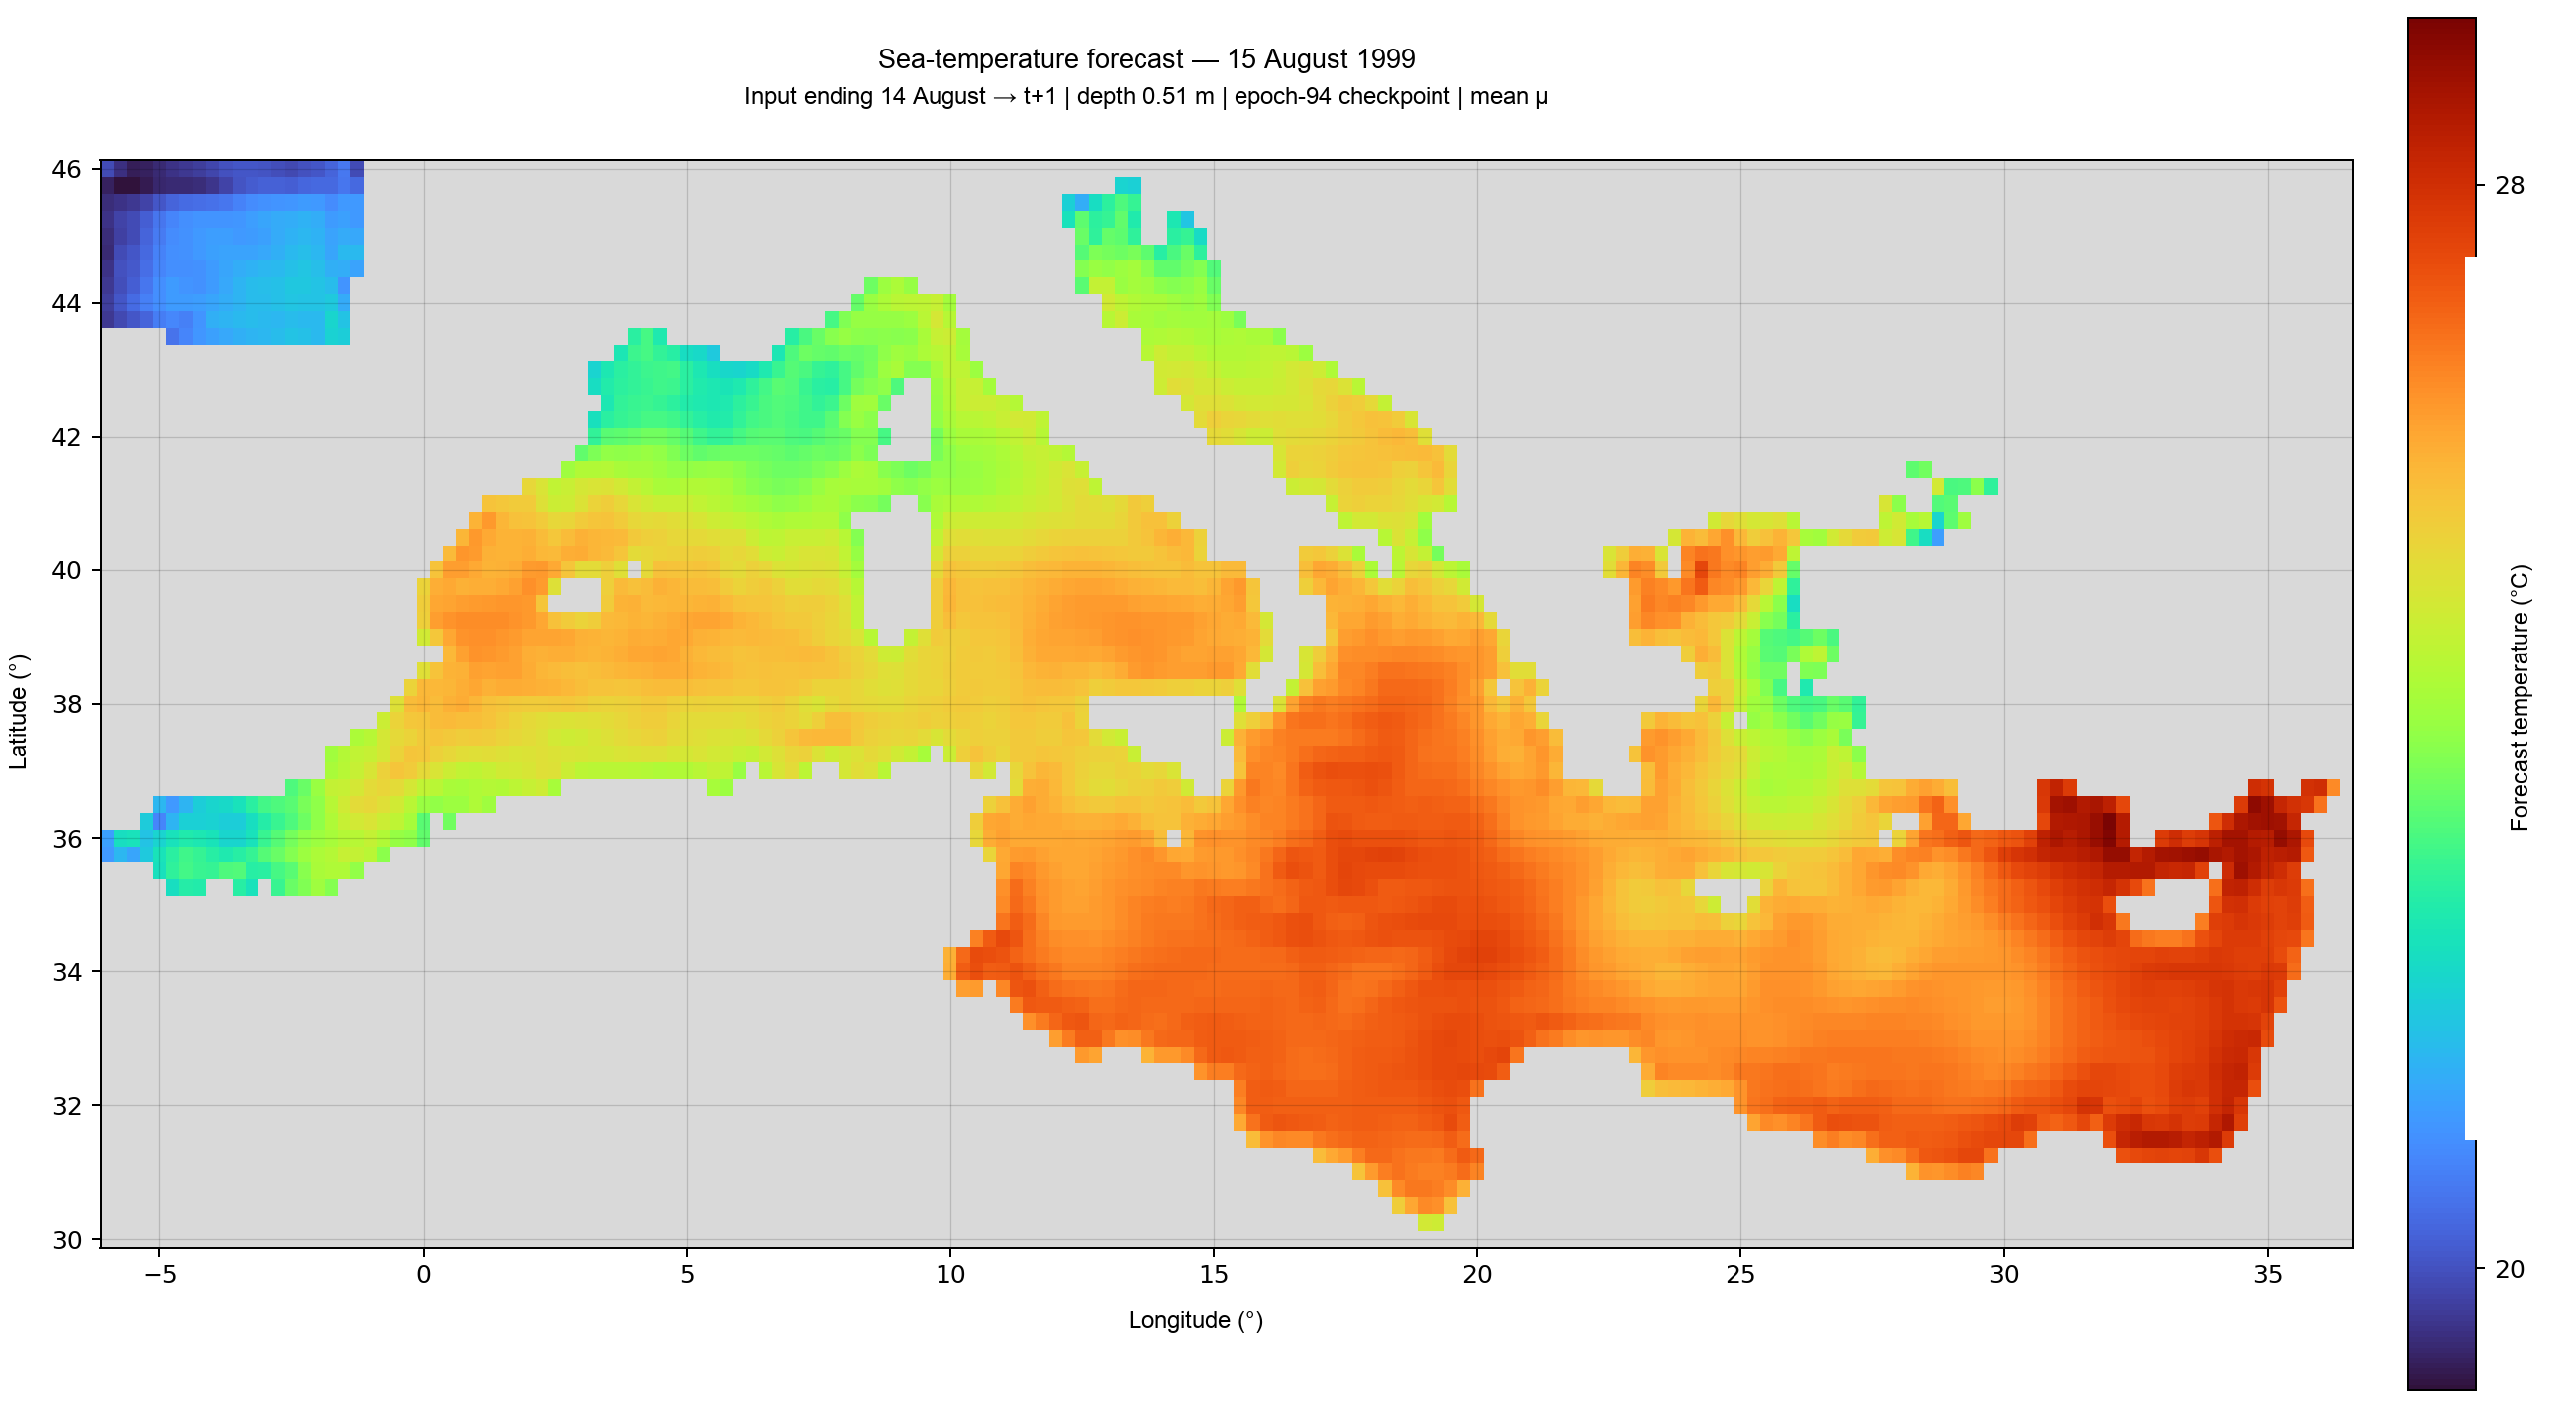
\includegraphics[width=\textwidth]{temperature-forecast-1999-08-15-english.png}
\caption{Forecast mean for potential temperature on 15 August 1999 at 0.506~m. The preceding three daily states form the input context. This panel displays the forecast only.}
\label{fig:temperature-forecast}
\end{figure}

For each surface grid point $p$ and variable $q$, the annual map is
\[
E_q(p)=\frac{1}{N_q(p)}\sum_{t=1}^{364}
\left|\widehat{y}_{q,t}(p)-y_{q,t}(p)\right|,
\]
where $N_q(p)$ counts only dates for which the target is valid. Land cells and cells with no valid target remain masked. Figure~\ref{fig:annual-mae} shows the four variables in separate panels with independent physical scales.

\begin{figure}[p]
\centering
\IfFileExists{img/annual-mae-maps-1999.png}{
  \includegraphics[width=\textwidth]{annual-mae-maps-1999.png}
}{
  \fbox{\parbox[c][6cm][c]{0.9\textwidth}{\centering Run the annual evaluator to generate \texttt{annual-mae-maps-1999.png}.}}
}
\caption{Pointwise mean absolute one-day forecast error over 364 targets from 2 January to 31 December 1999 at 0.506~m. Temperature, salinity, zonal velocity $u$, and meridional velocity $v$ use separate colour scales and their native physical units.}
\label{fig:annual-mae}
\end{figure}

The annual aggregation is more robust than a signed error map from one selected date: positive and negative residuals cannot cancel, while persistent coastal, frontal, or circulation-related error structures remain visible. The per-variable coverage values in Table~\ref{tab:physical-probabilistic-results} are marginal diagnostics; they should be interpreted together with mean predicted standard deviation and deterministic skill.

\section{Discussion}

The central experimental finding is robust across the two years and across normalized aggregate and physical temperature metrics: the compact 3D U-Net learns a plausible one-day mapping but does not improve on persistence. Three features of the setup help explain this result.

First, the target is the full next-day state. Most of that field is already contained in the latest input, so the network spends capacity reconstructing a large persistent component. Predicting $X_{t+1}-X_t$ and adding it back through a fixed residual path would make the learning problem focus on the smaller daily change while preserving persistence as the zero-increment solution.

Second, the six-year archive is small relative to the dimensionality of the output. After splitting, only 1,458 highly correlated daily training pairs are available. Each pair contains many grid cells, but those cells do not provide independent temporal examples of rare circulation and surface-forcing regimes. Increasing spatial sample count cannot substitute fully for longer temporal coverage.

Third, the model observes no atmospheric forcing, boundary tendency, or sea-surface-height input. Surface heat fluxes and wind stress strongly affect near-surface temperature and currents, while sea-surface-height gradients contain information about circulation. Their absence is particularly relevant to the large surface-temperature skill deficit. Incorporating them requires an architecture that fuses two-dimensional and three-dimensional fields without artificial vertical replication.

Other limitations concern the objective and evaluation. A single Gaussian per point cannot express multimodal futures or residual covariance. The fixed factor of two for temperature and for the auxiliary MSE was refined through a small number of runs rather than a systematic search. The aggregate normalized metric can conceal differences among salinity and velocity channels. These limitations define the next experiments rather than invalidating the implemented pipeline: data splitting, masking, normalization, resumable training, persistence comparison, and probabilistic diagnostics have all been verified end to end.

\chapter{Conclusions and Future Work}
\label{chap:conclusions}

\section{Achievements}

This thesis set out to design, implement, and evaluate an end-to-end deep-learning pipeline for probabilistic three-dimensional forecasting of the Mediterranean ocean state. The resulting system covers the complete path from a large Copernicus-derived NetCDF archive to reproducible full-year inference. It performs lazy Xarray/Dask data access, selects the relevant variables, applies a depth-dependent land--sea mask, creates chronological train--validation--test subsets, fits standardization statistics on training data alone, and constructs supervised PyTorch samples without loading the complete archive into memory.

The forecasting model is a compact 3D U-Net with 90,952 trainable parameters. Three consecutive daily states provide twelve input channels, and the network predicts four variables for the following day at 46 depth levels. The encoder and decoder jointly process depth, latitude, and longitude, while skip connections retain high-resolution information. Two output heads estimate a conditional mean and log-variance at every valid point. This design turns the model into a heteroscedastic Gaussian forecaster and permits deterministic errors and uncertainty intervals to be evaluated from the same output.

The training procedure is also a substantive result of the work. A target mask prevents land and invalid cells from influencing gradients. The objective combines Gaussian negative log-likelihood with a channel-weighted mean-squared-error term. AdamW optimization, gradient clipping, chronological validation, separate best and last checkpoints, resume support, end-of-epoch fixed-weight evaluation, and cumulative learning-curve generation make long Colab runs recoverable and auditable. The preserved checkpoints document the development from one to three context days and from a small to a wider latent representation.

The final model was selected at epoch 94. On 1998 validation data it obtained normalized RMSE 0.1783 and MAE 0.0843; on the unseen 1999 test year the corresponding values were 0.2013 and 0.0907. Near-surface temperature forecasts achieved a test RMSE of 0.419$^{\circ}$C and MAE of 0.277$^{\circ}$C. These values show that the network reconstructs physically plausible fields and learns beyond its initial state.

The most important conclusion is nevertheless negative: the predicted mean does not outperform persistence. Test persistence RMSE is 0.1943 in aggregate standardized space, yielding an RMSE skill of $-0.0736$. For near-surface temperature, persistence RMSE is 0.208$^{\circ}$C and neural skill is $-3.043$. Reporting this result directly is essential. The goal of an experimental thesis is not to guarantee a positive score, but to establish what the implemented method can and cannot achieve under a controlled protocol.

The uncertainty output provides a separate result. Test coverage is 0.748 for the nominal 68\% interval and 0.946 for the nominal 95\% interval. The wider interval is close to nominal coverage, while the one-standard-deviation interval contains too many targets and is therefore conservative on aggregate. Near-surface temperature intervals are more conservative still. These metrics show that the variance head learns a non-trivial scale, but coverage alone is only a partial calibration test and does not imply that complete sampled ocean states would be physically coherent.

\section{Limitations}

The first limitation is the temporal extent of the dataset. Six years produce only four years for training after reserving one year each for validation and test. Consecutive ocean states are highly correlated, so the large number of spatial values in one tensor does not create an equally large number of independent circulation regimes. Rare events, unusual atmospheric conditions, and interannual variability are only sparsely represented.

The second limitation is the forecast formulation. The network predicts the complete state one day ahead. At this horizon, the latest observed state is already an excellent approximation. A small smoothing error or bias can make a learned field worse than persistence even when the broad spatial structure is accurate. The current objective does not explicitly preserve the latest input or isolate the daily increment.

The third limitation is the set of predictors. Temperature, salinity, and horizontal velocities are used, but the network has no atmospheric forcing, surface fluxes, wind stress, bathymetry channel, or lateral-boundary input. Sea-surface height is selected and standardized by the pipeline but excluded from the volumetric model because it is two-dimensional. The strong surface-temperature deficit suggests that missing surface drivers are consequential.

The fourth limitation is probabilistic. Independent Gaussian outputs cannot represent skewed or multimodal residuals, correlations between variables, or coherent displacement of fronts and eddies. The learned variance also mixes irreducible variability, omitted predictors, and model error. It does not quantify uncertainty over the network parameters. Therefore, the system should not be interpreted as a complete ensemble forecast.

The fifth limitation is experimental scale. Hyperparameters were refined through a small sequence of checkpoints rather than a controlled factorial or Bayesian search. The final configuration changes more than one element relative to earlier checkpoints, preventing a causal attribution of improvement to context length alone. The historical training logs also did not preserve the exact GPU, elapsed compute time, maximum epoch argument, patience, and original package versions. The final software should record these fields automatically.

Finally, the aggregate standardized metrics pool all variables and depths. This is useful for model selection but incomplete for oceanographic interpretation. Physical-unit results were preserved for temperature only. Salinity and velocity should receive separate diagnostics, including vertical profiles and regional maps, before the model is used to support scientific conclusions.

\section{Future Work}

The first modelling change should make persistence part of the architecture. Instead of predicting $X_{t+1}$ directly, the network can predict the increment

\[
\Delta X_{t+1}=X_{t+1}-X_t,
\qquad
\widehat{X}_{t+1}=X_t+\widehat{\Delta X}_{t+1}.
\]

With this residual formulation, a zero network output exactly reproduces persistence. Optimization can focus on the smaller and dynamically meaningful change, and negative skill should become easier to diagnose by variable and region. Separate loss weights by variable and depth could then prevent the many deep, slowly varying cells from dominating objectives intended to improve surface dynamics.

A second priority is a longer and more diverse dataset. Extending the GLORYS12-derived archive beyond six years would expose the model to more seasonal cycles and circulation regimes. A proper experiment should preserve a final chronological test block and perform hyperparameter selection only on earlier years. Training on the native or a less coarsened grid may retain mesoscale structures, although memory and compute requirements would increase sharply.

The predictor set should also be expanded. Atmospheric variables such as wind components, surface-air temperature, pressure, radiation, precipitation, and heat flux can inform daily surface changes. Sea-surface height and mixed-layer depth can be introduced through a two-dimensional encoder whose features are fused with the three-dimensional volume at selected depths or latent resolutions. Static bathymetry and coordinate encodings may help distinguish physically different boundary regions that otherwise share similar local patches.

Longer forecast horizons are needed to determine when a learned model becomes more useful than persistence. Direct models could predict several lead times, or the one-day network could be evaluated autoregressively. Autoregression requires dedicated stability analysis because small biases accumulate and predictions leave the training distribution. Multi-step training, scheduled sampling, or losses evaluated over trajectories may reduce this mismatch.

Architecturally, 3D attention or neural-operator blocks could enlarge the receptive field beyond the compact convolutional hierarchy. Mediterranean circulation contains interactions across basins and through narrow straits that may not be captured adequately by local convolutions. Such additions should be compared through controlled ablations, retaining the same dataset split and persistence reference so that increased complexity is justified by measurable skill.

The probabilistic model can be improved along two complementary paths. Ensembles obtained from independently trained networks, bootstrapped data, or dropout-based approximations can probe epistemic uncertainty. Conditional diffusion or other generative approaches can produce spatially coherent alternative trajectories and represent non-Gaussian distributions. These methods require proper scoring rules such as CRPS or energy score, rank histograms, reliability diagrams by depth and region, and comparisons of both calibration and sharpness.

The evaluation software should accumulate physical-unit RMSE, MAE, bias, and uncertainty for every output variable and depth. Vertical profiles, seasonal subsets, and maps of median and extreme-error cases would reveal where improvement occurs. Independent observations would provide a stronger test than reanalysis targets alone. Automated case selection would also prevent qualitative figures from being chosen after inspecting their visual appearance.

Finally, reproducibility metadata should become part of every checkpoint. The command-line arguments, Git commit, product identifier, data checksum, mask checksum, Python and library versions, GPU name and memory, session duration, and cumulative training time can all be stored with negligible overhead. This would close the remaining provenance gaps in the present experiment and make later comparisons between architectures scientifically defensible.

The current system therefore provides a complete and verified baseline. Its negative skill against persistence identifies the most important technical problem rather than concealing it. The pipeline, checkpoints, and evaluation metrics establish a foundation on which residual prediction, additional forcings, longer archives, stronger architectures, and richer probabilistic methods can be tested one change at a time.

\backmatter
\bibliographystyle{unsrtnat}
\bibliography{reference}
\end{document}
